\subsection{Kompozice}

\subsubsection{Menu}
Inspirace pro menu vycházela z kompozice, která se už používala na stránce s Travel Buddy administrací. Protože ale nebyla uzpůsobená na to, aby se používala jinde, bylo na mě ji to „naučit“.

Mé nové menu bylo složené ze dvou části. První, horní, byla samotná navigace. Ta se od té původní zase tolik nelišila, jen jsem podle designu trochu upravil barvy. Jinak se jednalo o malou komponentu, do které šel vložit text, ikona, odkaz, akce po kliknutí, a zda je aktivní. Vše ovládala rodičovská komponenta AppMenu (pro desktop) nebo její potomek MenuRight (pro mobil), obě k tlačítkům ještě přidaly klíč, aby je React zvládnul lépe vykreslit. Druhá komponenta byl obrázek uživatele s jeho jménem a textem pro odhlášení. Přes ni byl daný odkaz, po jehož kliknutí byl uživatel odhlášen a vrácen na domovskou stránku.

Desktopovou verzi asi nemusím příliš popisovat. Horní část byla ve ScrollShadow komponentě, což poslední odkazy dokázalo skrýt, pokud by jich bylo hodně a nevešly by se na obrazovku. Zajímavější je ovšem verze pro mobil. Je totiž založená na již zmíněné SwipeableDrawer komponentě a dá se ovládat změnou proměnné open.

Pokud toto menu chcete kdekoliv použít, stačí mu předat menuItems parametr, složený z pole obsahujícího text na tlačítko, odkaz, ikonu a zda je aktivní (k tomu mi skvěle poslouží Next.js hook usePathname(), který vrací aktuální url). Změny, které se promění čistě na mobilu, zase předávám parametry isOpen, akci po zavření onClose a titulkem header.

\begin{figure}
    \centering
    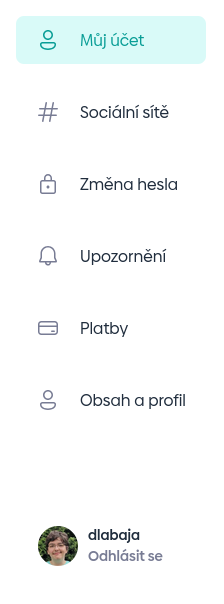
\includegraphics[width=0.5\linewidth]{obrazky/menu.png}
    \caption{Menu}
\end{figure}


\subsubsection{Account Container}
Protože má každá z podstránek stejnou horní část, a také, aby se mi lépe umisťovaly, vytvořil jsem pro každou z nich kontejner. Ten si podle aktuální cesty tvoří jméno stránky a v mobilní verzi se mu objevuje tlačítko, kterým se dá otevírat postranní menu. Do komponenty samotné se pak vkládají jednotlivé stránky, které Vám nyní představím.


\subsubsection{Podstránka Můj účet}
Stránka s účtem se dá označit jako srdce celého nastavení. Na první pohled Vás určitě zaujal banner přes celou stránku, o kterém již byla řeč. Jediný rozdíl oproti tomu na profilu je jeho výška, která je o 100 pixelů kratší. Hned pod ním se dá nastavit profilový obrázek.

Kromě toho jde na této stránce nastavit jméno, příjmení, přezdívku, pod čím chcete vystupovat, email, telefon, a sekci O mně, ve které se můžeme představit.

Ačkoliv komponenta s názvem města Olomouc vypadá jako jen další Text box, není tomu tak. Pokud do ní totiž začnete psát, začnou se vám díky Google Autocomplete funkci zobrazovat návrhy měst (případně i míst). Box vlastně ani neobsahuje text, ale objekt, jehož součástí jsou i GPS souřadnice daného místa.

Posledním boxem je již zmiňovaný Combo box se všemi státy světa.

Na konci celého nastavení leží tzv. Bookmark komponenta. Když ji rozbalíte, dostanete možnost odstranit Váš účet z Worldee.

Po kliknutí na tlačítko se otevře Modal – takové malé plovoucí okno. Tento konkrétní lze zavřít jen kliknutím na horní křížek nebo jedním ze dvou spodních tlačítek. Uvnitř jsou checkboxy, ve kterých uživatel vybere, proč chce Worldee opustit. Také může dolů do Text boxu napsat konkrétní důvod. Dole pak už jen potvrdí své heslo (pokud ho má) a kliknutím na tlačítko „Opustit Worldee“ bude odhlášen a přesměrován na hlavní stránku.

\begin{figure}
    \centering
    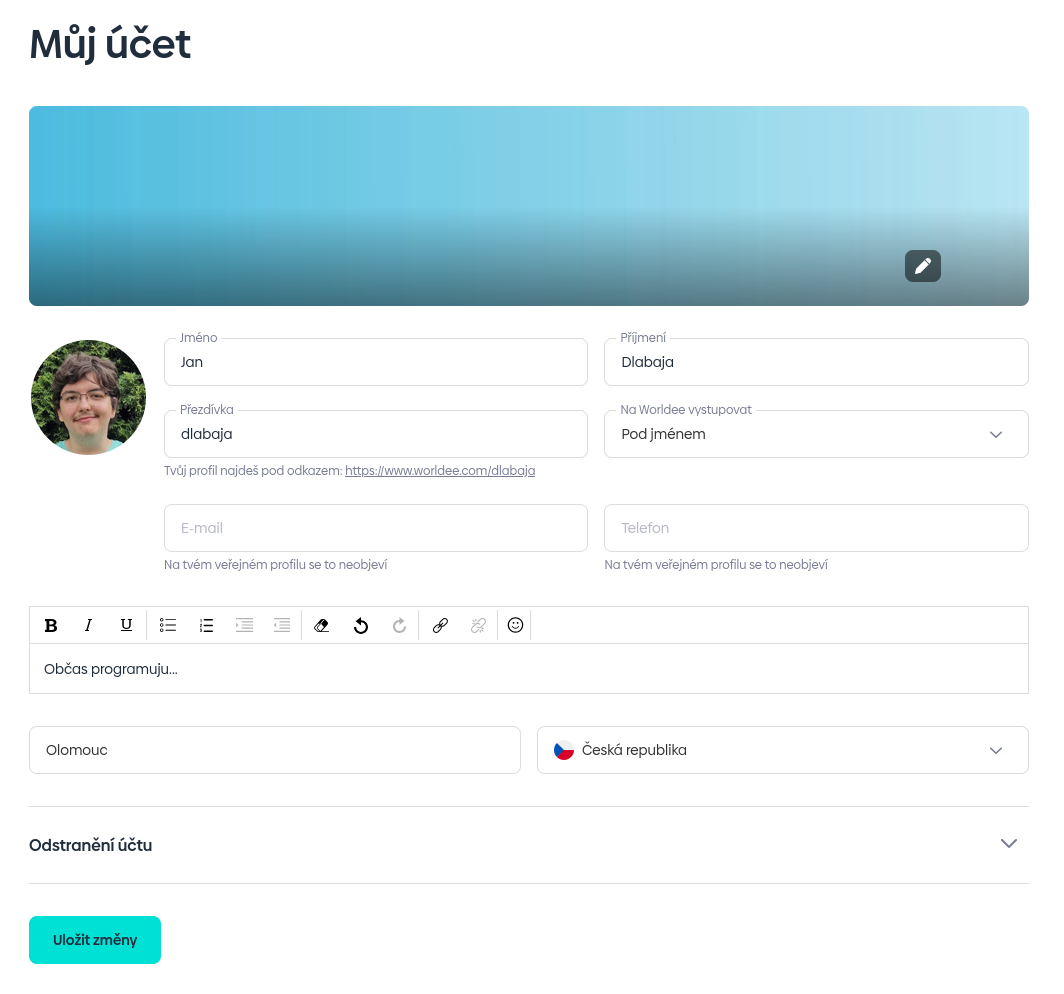
\includegraphics[width=1\linewidth]{obrazky/account.png}
    \caption{Podstránka Můj účet}
\end{figure}

\begin{figure}
    \centering
    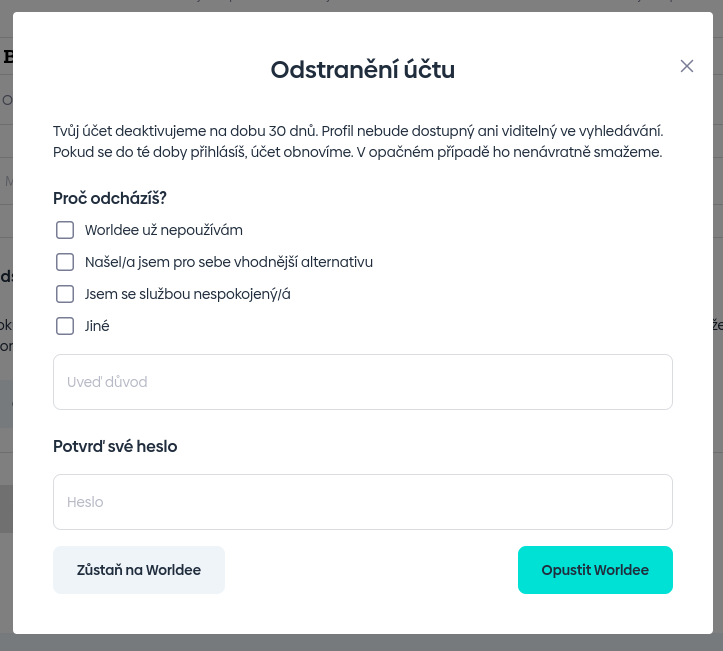
\includegraphics[width=1\linewidth]{obrazky/delete_account.png}
    \caption{Dialog s odstraněním účtu}
\end{figure}


\newpage
\subsubsection{Podstránka Sociální sítě}
Na této stránce si s Worldee můžete propojit svůj Facebook nebo Instagram účet, který se Vám pak objeví na profilu. Každá sociální síť se skládá z názvu, levé části a tlačítka. Pokud jste si ji zatím nepřipojili, bude levá část pouze Text box a pravá tlačítko „Propojit účet“. Pro propojení stačí napsat URL Vašeho profilu na jedné z těchto sítí. Pokud bylo úspěšné, Text box se změní na komponentu složenou z ikony a dvou textů oznamujících, že je účet propojen, a z původně zeleného tlačítko se stane tmavě šedé s názvem „Zrušit propojení“.

\begin{figure}[!h]
    \centering
    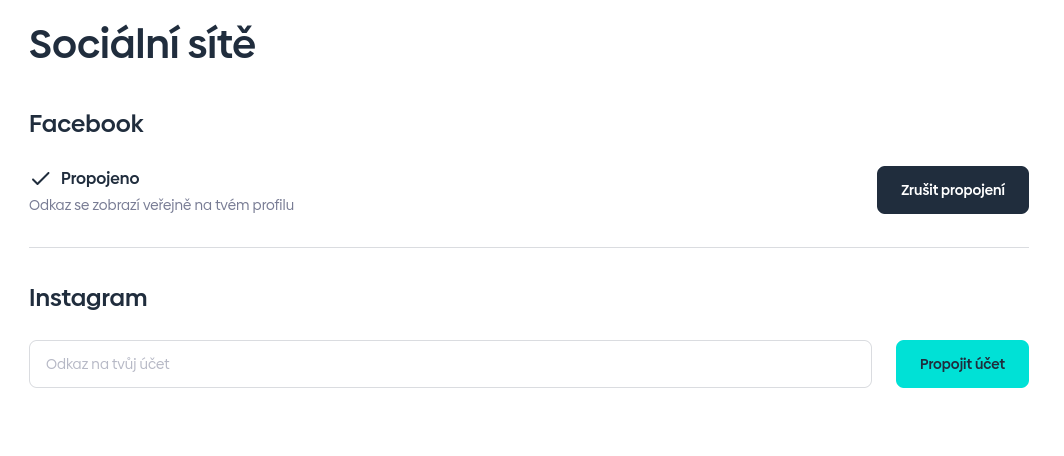
\includegraphics[width=1\linewidth]{obrazky/social_networks.png}
    \caption{Podstránka Sociální sítě}
\end{figure}


\newpage
\subsubsection{Podstránka Změna hesla}
Zatím jedna z těch jednodušších stránek – pouhá tři pole, jejichž typ je nastaven jako heslo, a text. Pokud jste přihlášeni přes přes službu třetí strany jako třeba Google, první pole se vám neukáže – ještě u nás totiž žádné heslo nemáte. Objeví se až po nastavení nového.

\begin{figure}[!h]
    \centering
    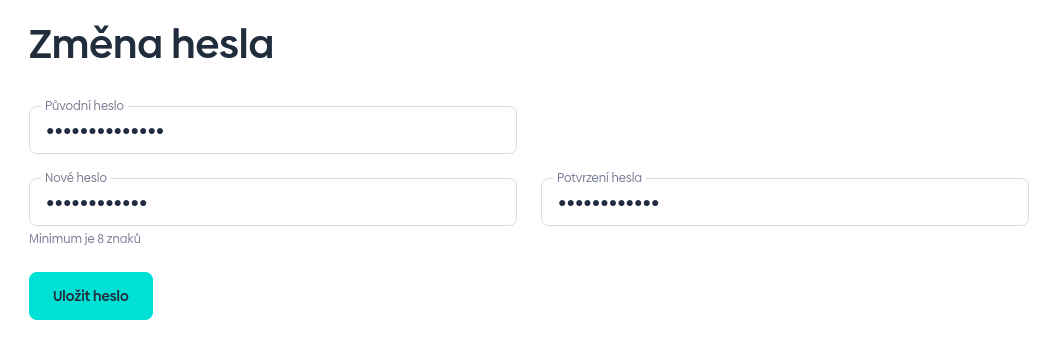
\includegraphics[width=1\linewidth]{obrazky/change_password.png}
    \caption{Podstránka Změna hesla}
\end{figure}


\newpage
\subsubsection{Podstránka Upozornění}
Tato kompozice se skládá ze dvou částí. Ta levá je velmi podobná té ze Sociálních sítí – jen má jiný obsah. Napravo je ale toggle tlačítko, kterým si uživatel může nastavit, z čeho chce (nebo nechce) dostávat webová upozornění.

\begin{figure}[!h]
    \centering
    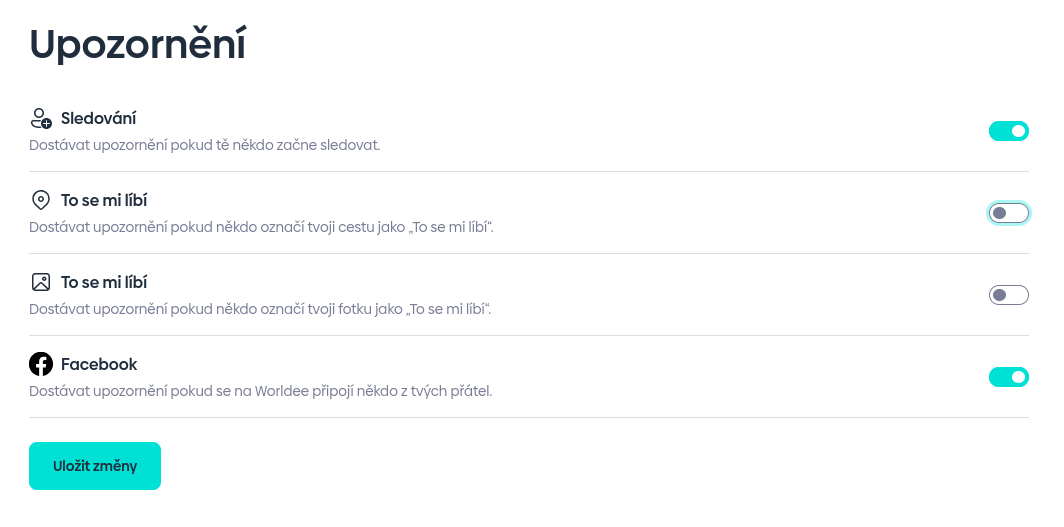
\includegraphics[width=1\linewidth]{obrazky/notify_settings.png}
    \caption{Podstránka Upozornění}
\end{figure}


\newpage
\subsubsection{Podstránka Obsah a profil}
A nyní poslední mnou vytvořená stránka. Je tvořená sekcí Profil a Zobrazení obsahu. V té první si můžete již známými Combo boxy vybrat, zda chcete, aby byl Váš profil viditelný pro všechny nebo jen pro vás. Hned vedle zase asijští zákazníci mohou přepnout střed mapy z Evropy na Asii.

Pod komponentami se nacházejí dva toggly. U horního si nastavíte, zda chcete schvalovat, když Vás někdo označí na jakékoliv fotografii, než se toto označení zobrazí na vašem profilu. Druhý toggle už se nachází v sekci Zobrazení obsahu a umožňuje Vám nejnovější cesty na Worldee zobrazovat ve feedu.

\begin{figure}[!h]
    \centering
    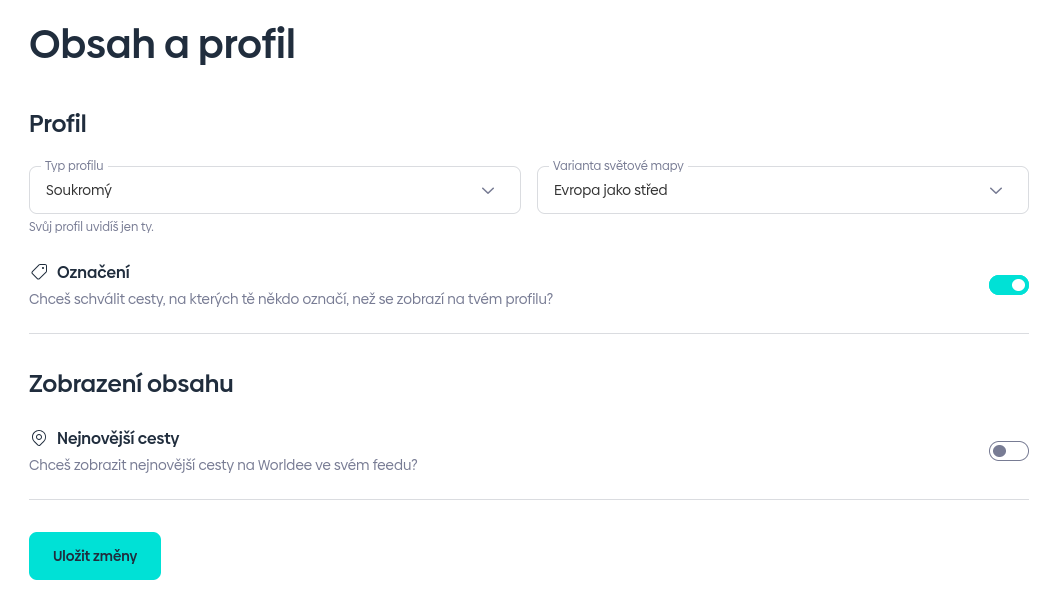
\includegraphics[width=1\linewidth]{obrazky/content_and_profile.png}
    \caption{Podstránka Obsah a profil}
\end{figure}


\newpage
\subsubsection{Podstránka Platby}
Poslední stránkou na seznamu je ta s platbami. Jako jedinou jsem ji nemusel psát úplně od základů, nicméně pár úprav bylo pro zakomponování do systému potřeba. Všechny className atributy jsem přesunul do <div /> elementů, načítání dat jsem připojil ke svému systému načítání stránky a proběhlo tak až po prvním renderu komponenty, a zmizela i přehnaně komplexní logika pro zobrazení plateb.
\\
\begin{figure}[!h]
    \centering
    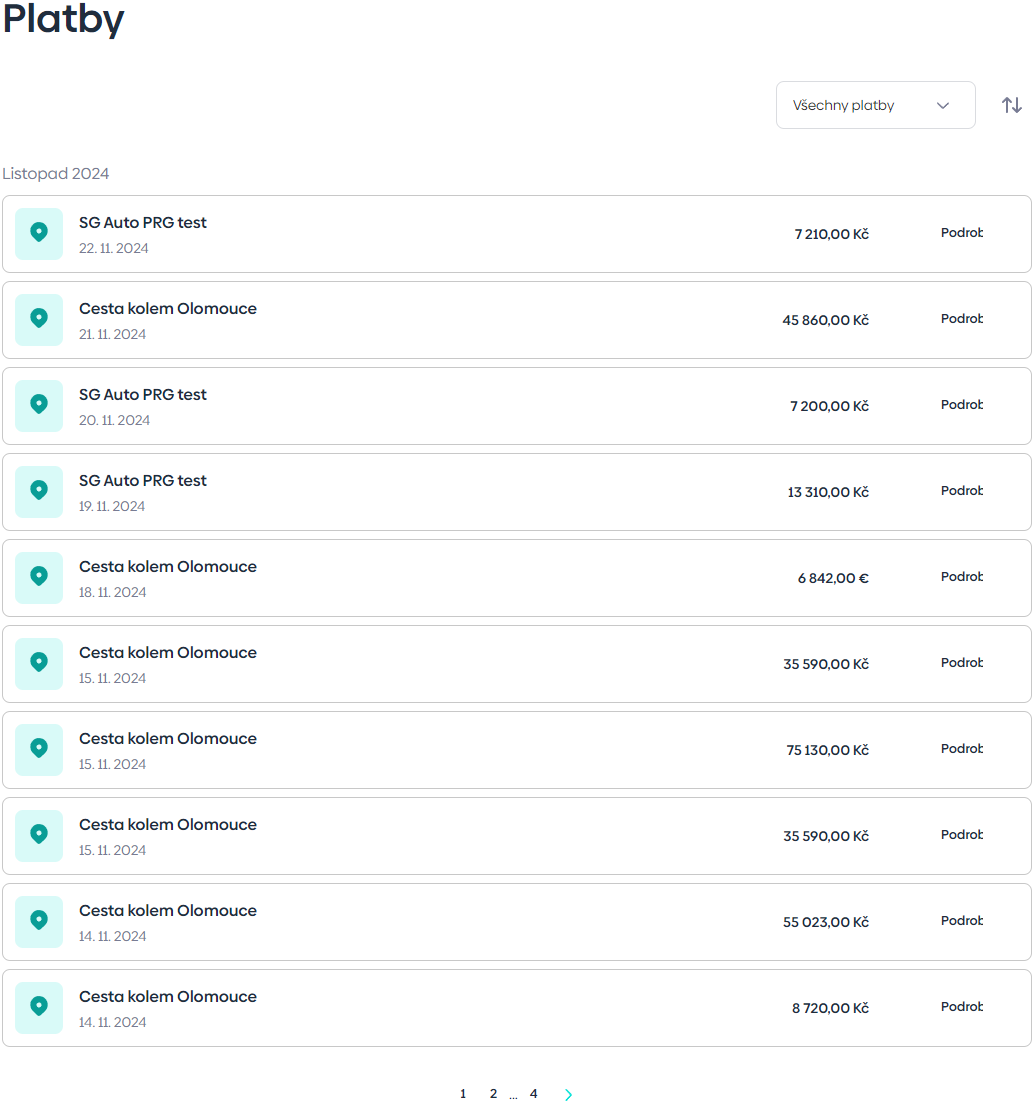
\includegraphics[width=0.9\linewidth]{obrazky/platby.png}
    \caption{Podstránka Platby}
    \label{fig:enter-label}
\end{figure}